
%we experiment with the dataset proposed by \cite{luo2016temporal} which aims at extracting relations between entity and time. With some heuristics, this dataset can be further split intro three subsets with different levels of reliability, which enables us to conduct all our experiment settings. To show the generalization ability of our model, we also experiment with the dataset proposed by \cite{riedel2010modeling}, which aims at extracting relations between entities and there is no prior knowledge of the data quality can be used. \todo{can be shorter}

%We also consider two types of relation extraction tasks. The first task aims at extracting relations between entity and time. Specifically, it requires the object to be an time expression and the subject to be an entity. As suggested by \cite{luo2016temporal}, the distant supervision dataset in this task can be naturally divided into several subsets with different levels of reliability. The basic idea is that number of important things related to one entity increases as the time scope becomes larger. For example, a sentence containing both \emph{Alphabet} and \emph{October\_2\_2015} is very likely to express the foundation time of \emph{Alphabet}, while a sentence containing both \emph{Alphabet} and \emph{2015} may instead talk about its financial report of year 2015. We experiment with this task because it has a public dataset that contains both reliable and unreliable data, which enables us to conduct all of our experiments.

%The second task aims at extracting relations between entities, which is extensively studied in relation extraction. We experiment with this task to see if our transition matrix method generalizes well in different datasets.

\begin{figure}[t!]
\begin{center}
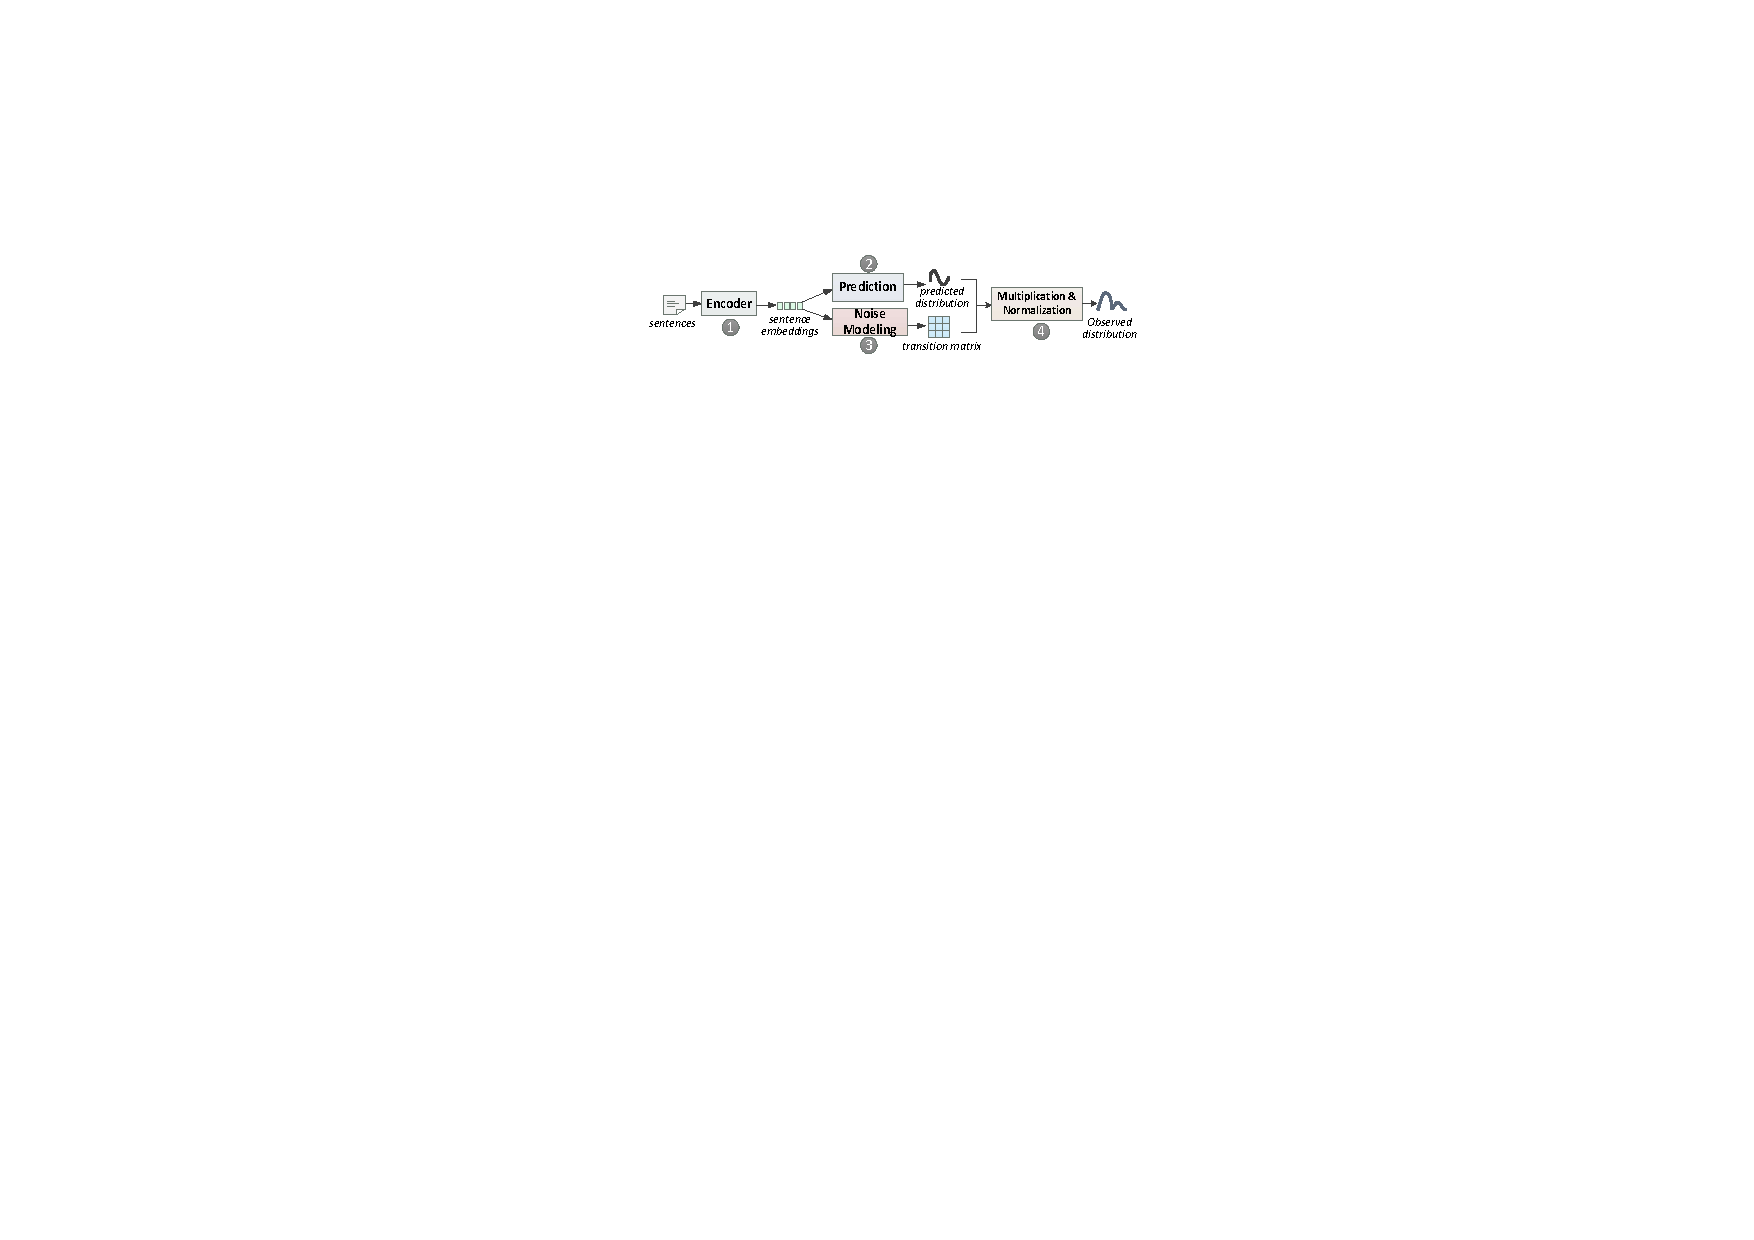
\includegraphics[width=0.5\textwidth]{figures/overview.pdf}	
\caption{Overview of our approach}
\label{fig: denoise_framework}
\end{center}
\end{figure}


\section{Our approach}\label{sec:approach}
%Our approach for distantly supervised relation extraction is depicted in Figure \ref{fig: denoise_framework}.
%First, the input sentence (or sentence
%bag) is passed to a sentence encoder to get sentence embedding(s). After that, the model is split into two branches.
%The prediction branch generates the predicted relation distribution $\mathbf{p}$ of the input sentence (or sentence
%bag). The noise modeling branch generates the transition matrix $\mathbf{T}$. Finally, the predicted distribution is
%multiplied by the transition distribution to generate the observed relation distribution $\mathbf{o}$. The predicted
%relation distribution $\mathbf{p}$ is the output of the model while the observed relation distribution $\mathbf{o}$ is
%used to simulate the relation assigned by distant supervision. In this way, the noise is modeled by the transition
%matrix and the real
%prediction is protected from the influence of the noise. In rest of this section, we will first describe the sentence level model, and then extend the model to bag level.
%
%\subsection{Sentence Encoder}
%The sentence encoder serves to transform an input sentence to an embedding vector that encodes semantic meaning of the sentence. Theoretically, almost any sentence encoder would work here. Similar to previous researches, we also use the piecewise convolutional neural network (PCNN) model \cite{zeng2015distant} as our sentence encoder. First, the distances of each word to the subject and the object are embedded as randomly initialized vectors and concatenated to the original word vector. After that, the PCNN model divides the input sentence into three pieces by the subject and the object, and apply convolutional neural network (CNN) to each piece to calculate the piece embedding. The final sentence embedding is the concatenation of the embeddings of the three pieces.

In order to deal with the noisy training data obtained through \DS, our approach follows four steps as depicted in Figure \ref{fig: denoise_framework}.
First, each input sentence is fed to a sentence encoder to generate an embedding vector. Our model then takes the sentence embeddings as input and produce a predicted relation
distribution, $\mathbf{p}$, for the input sentence (or the input sentence bag). At the same time, our model dynamically produces
a transition matrix, $\mathbf{T}$, which is used to characterize the noise level of the \DS-labeled input sentence (or the
bag). Finally, the predicted distribution is multiplied by the transition matrix to produce the observed relation
distribution, $\mathbf{o}$. This observed distribution $\mathbf{o}$ is used to capture the (possibly noisy) relation labels
assigned by \DS and update our model parameters during training, while the predicted relation distribution $\mathbf{p}$ is
the output of our model during testing.
One of the key challenges of our approach is
on determining the weights of the transition matrix, $\mathbf{T}$, which will be described in Section~\ref{sec:training}.
%In the remainder of this section, we will describe how our approach can be applied to sentence- and bag-level models.



\subsection{Sentence-level Modeling}

\paragraph{Sentence Embedding and Prediction}
 In this work, we use a piecewise convolutional neural network~\cite{zeng2015distant} for sentence encoding, but other sentence embedding models can also be used.
%We use a model similar to the one presented in \cite{luo2016temporal} for distribution prediction at the sentence level.
To generate the predicted relation distribution, $\mathbf{p}$,  we first feed the sentence embedding to a full connection layer, and then use \emph{softmax} for
relation classification. Again, other probabilistic prediction methods can also be used here.

\paragraph{Noise Modeling}
%The noise modeling branch calculates a transition matrix dynamically for each sentence (or sentence bag) to model its noise pattern.

We use a fully connected layer in the neural network to perform noise
modeling at the sentence level. Each sentence embedding, $\mathbf{x}$,
generated by the encoder is passed to the full connection layer as a  non-linearity to obtain the
sentence embedding $\mathbf{x}_n$ used specifically for the noise modeling
branch.
%\todo{ZW: What's the difference between  $\mathbf{x}$ and $\mathbf{x}_n$}.
 We then use a \emph{softmax} to calculate the transition matrix, $\mathbf{T}$, for each sentence:
%
%the sentence embedding $\mathbf{x}$ is passed to another full connection layer to obtain the sentence embedding $\mathbf{x}_n$ used specifically for noise modeling branch. The transition matrix $\mathbf{T}$ is calculated using softmax function :
\begin{equation}\label{eq_tm}
T_{ij} = \frac{exp({\mathbf{w}_{ij}^T \mathbf{x}_n + b})}{\sum_{j=1}^{|\mathbb{C}|}{exp({\mathbf{w}_{ij}^T \mathbf{x}_n + b}})}
\end{equation}
where $T_{ij}$ is the conditional probability for the given sentence to be labeled as relation $j$ by \DS, but with $i$ as the true relation, $b$ a scalar bias,  $|\mathbb{C}|$ the number of relations, $\mathbf{w}_{ij}$ is a shared weight vector to characterize the confusion between $i$ and~$j$. %, shared across the dataset.
%The \emph{softmax} function guarantees that each row of $\mathbf{T}$ sums to 1.

\blue{----F: Dynamic v.s. Static:  Here, we dynamically produce a transition matrix, $\mathbf{T}$, specifically for each sentence, but with the parameters ($\mathbf{w}_{ij}$) shared across the dataset. By doing so, we are able to adaptively characterize  the noise level for each sentence, with a few parameters only. In contrast, one could also produce one single transition matrix for all sentences, with much less computation, where one need not to compute $\mathbf{T}$ on the air.}




\paragraph{Observed Distribution}
When we model the noise with a transition matrix,
if the true relation of an input training instance is $i$, we can assume that this relation $i$ could be labeled as relation $j$ by \DS  with probability $T_{ij}$. Therefore, we can model the observed relation distribution, $\mathbf{o}$, by
multiplying transition matrix, $\mathbf{T}$, and the predicted relation distribution, $\mathbf{p}$:
 \begin{equation}
\mathbf{o} = \mathbf{T}^T \bm\cdot \mathbf{p}
\label{eq_transition}
 \end{equation}
 \iffalse
 \begin{equation}
 \label{norm_o}
 o_i = \frac{o_i}{\sum_i{o_i}}
 \end{equation}
 \fi
where $\bm\cdot$ represents dot product, and we normalize the elements of $\mathbf{o}$ to ensure $\sum_i{o_i}=1$.

Different from previous works that use the predicted relation distribution $\mathbf{p}$ to directly \red{match} the relation labeled by \DS\red{~\cite{zeng2015distant,lin2016neural}??}. We instead use $\mathbf{o}$ to match the noisy label during training and still use $\mathbf{p}$ as output during testing.
By doing so, we can see that Equation \ref{eq_transition} actually models the procedure of how the noisy label is produced and thus protects $\mathbf{p}$ from the noise.
%can help the model make better use of the noisy training data. \red{How to better use?? by using regularization????}
%Also note that the noise modeling branch and $\mathbf{o}$ is only used in the training phase. In the test phase, we only use the prediction branch and take the predicted relation distribution $\mathbf{p}$ as our output. \todo{last paragraph can be removed}

\subsection{Bag Level Modeling}
\paragraph{Bag Embedding and Prediction}
One of the key challenges for bag level model is how to aggregate the embeddings of individual sentences of the bag.
In this work, we experiment two methods, namely average and attention aggregation~\cite{lin2016neural}.
%The average aggregation
The former calculates the bag embedding, $\mathbf{s}$, by averaging the embeddings of each sentence, and  then feed it to a \emph{softmax} classifier for relation classification.

The attention aggregation calculates an attention value, $a_{ij}$, for each sentence $i$ in the bag with respect to each relation $j$, and aggregates to  the bag level as  $\mathbf{s}_j$, by the following equations\footnote{While~\cite{lin2016neural} use bilinear function to calculate $a_{ij}$ in their paper, we simply use dot product since we find these two functions perform similarly.}:

\begin{equation}
\begin{aligned}
\mathbf{s}_j = \sum_i^{n}{a_{ij} \mathbf{x}_{i}}
\end{aligned}
\label{att_sum}
\end{equation}

\begin{equation}
\begin{aligned}
a_{ij} = \frac{exp(\mathbf{x}_i^T \mathbf{r}_j)}{\sum_i^n{exp(\mathbf{x}_i^T \mathbf{r}_j)}}
\end{aligned}
\label{cal_att}
\end{equation}
where $\mathbf{x}_{i}$ is the embedding of sentence $i$, $n$ the number of sentences in the bag, and $\mathbf{r}_j$ is the randomly initialized embedding of relation $j$.
% and $\alpha_{ij}$ is the attention value over sentence $i$ with respect to relation $j$.
Following~\cite{lin2016neural}, the resultant bag embedding $\mathbf{s}_j$ is fed to a \emph{softmax} classifier to predict the probability of relation $j$. \blue{this is a binary classifier, right???} \orange{no, multi-class classifier}

\paragraph{Noise Modeling}
\orange{Since the transition matrix models the transition distribution with respect to each true relation, the attention mechanism appears to be a natural fit for calculating the transition matrix in bag level. Similar to attention aggregation, we concentrate on each relation one by one and calculate its transition distribution respectively.}
Specifically, we calculate the bag embedding with respect to each relation using Equation \ref{att_sum} and \ref{cal_att} but with another set of relation embeddings $\mathbf{r}_t^j$.
We then calculate the transition matrix, $\mathbf{T}$, by:
\begin{equation}
T_{ij} = \frac{exp({\mathbf{s}_i^T \mathbf{r}_t^j  + b})}{\sum_{j=1}^{|\mathbb{C}|}{exp(\mathbf{s}_i^T \mathbf{r}_t^j + b})}
\end{equation}
where $\mathbf{s}_i$ is the bag embedding with respect to relation $i$, and $\mathbf{r}_t^j$ is the same embedding of relation $j$.
\orange{do we need to clarify that avg and att share the same noise modeling method?}
% We use an attention based mechanism to generate the transition matrix %for both average and attention aggregation models.
% for each sentence bag.

